\documentclass{beamer}

\usepackage[utf8]{inputenc}
\usepackage[brazil]{babel}

\usepackage{verbatim}

\usepackage{graphicx}

\usepackage{listings}
\usepackage{color}

\definecolor{mygreen}{rgb}{0,0.6,0}
\definecolor{mygray}{rgb}{0.5,0.5,0.5}
\definecolor{mymauve}{rgb}{0.58,0,0.82}
\definecolor{mybckg}{rgb}{0.95,0.95,0.95}
\lstset{
  backgroundcolor=\color{mybckg},  % choose the background color; you must add \usepackage{color} or \usepackage{xcolor}
  basicstyle=\footnotesize,       % the size of the fonts that are used for the code
  breakatwhitespace=false,         % sets if automatic breaks should only happen at whitespace
  breaklines=true,                 % sets automatic line breaking
  %captionpos=b,                    % sets the caption-position to bottom
  %commentstyle=\color{mygreen},    % comment style
  deletekeywords={...},            % if you want to delete keywords from the given language
  escapeinside={\%*}{*)},          % if you want to add LaTeX within your code
  extendedchars=true,              % lets you use non-ASCII characters; for 8-bits encodings only, does not work with UTF-8
  frame=single,                    % adds a frame around the code
  keepspaces=true,                 % keeps spaces in text, useful for keeping indentation of code (possibly needs columns=flexible)
  columns=flexible,
  %keywordstyle=\color{blue},       % keyword style
  %language=bash,                   % the language of the code
  morekeywords={*,...,Hello,LS,Update},            % if you want to add more keywords to the set
  %numbers=left,                    % where to put the line-numbers; possible values are (none, left, right)
  %numbersep=5pt,                   % how far the line-numbers are from the code
  %numberstyle=\tiny\color{mygray}, % the style that is used for the line-numbers
  rulecolor=\color{black},         % if not set, the frame-color may be changed on line-breaks within not-black text (e.g. comments (green here))
  %showspaces=false,                % show spaces everywhere adding particular underscores; it overrides 'showstringspaces'
  %showstringspaces=false,          % underline spaces within strings only
  %showtabs=false,                  % show tabs within strings adding particular underscores
  %stepnumber=2,                    % the step between two line-numbers. If it's 1, each line will be numbered
  %stringstyle=\color{mymauve},     % string literal style
  tabsize=2,                       % sets default tabsize to 2 spaces
  %title=\lstname                   % show the filename of files included with \lstinputlisting; also try caption instead of title
  literate=
  {á}{{\'a}}1 {é}{{\'e}}1 {í}{{\'i}}1 {ó}{{\'o}}1 {ú}{{\'u}}1
  {Á}{{\'A}}1 {É}{{\'E}}1 {Í}{{\'I}}1 {Ó}{{\'O}}1 {Ú}{{\'U}}1
  {à}{{\`a}}1 {è}{{\'e}}1 {ì}{{\`i}}1 {ò}{{\`o}}1 {ù}{{\`u}}1
  {À}{{\`A}}1 {È}{{\'E}}1 {Ì}{{\`I}}1 {Ò}{{\`O}}1 {Ù}{{\`U}}1
  {ä}{{\"a}}1 {ë}{{\"e}}1 {ï}{{\"i}}1 {ö}{{\"o}}1 {ü}{{\"u}}1
  {Ä}{{\"A}}1 {Ë}{{\"E}}1 {Ï}{{\"I}}1 {Ö}{{\"O}}1 {Ü}{{\"U}}1
  {â}{{\^a}}1 {ê}{{\^e}}1 {î}{{\^i}}1 {ô}{{\^o}}1 {û}{{\^u}}1
  {Â}{{\^A}}1 {Ê}{{\^E}}1 {Î}{{\^I}}1 {Ô}{{\^O}}1 {Û}{{\^U}}1
  {œ}{{\oe}}1 {Œ}{{\OE}}1 {æ}{{\ae}}1 {Æ}{{\AE}}1 {ß}{{\ss}}1
  {ç}{{\c c}}1 {Ç}{{\c C}}1 {ø}{{\o}}1 {å}{{\r a}}1 {Å}{{\r A}}1
  {€}{{\EUR}}1 {£}{{\pounds}}1,
  %basicstyle=\ttfamily
}

\useoutertheme{infolines} % add a footline 
\usetheme{Frankfurt}
%\setbeamertemplate{items}[square] % changes the markers, ball: 3-dimensional balls, circle: 2-dimensional (flat) circles, rectangle: rectangles, default: triangles 
%\setbeamertemplate{section in toc}[circle]
\setbeamertemplate{section in toc}[ball unnumbered]
\setbeamertemplate{enumerate item}[square]
\setbeamertemplate{itemize item}[triangle]
\setbeamertemplate{itemize subitem}[circle]
\setbeamertemplate{blocks}[rounded][shadow=true] % add rounded corners and a shadow to the box that surrounds the theorem
\setbeamertemplate{navigation symbols}{} % disable the drawing of navigation icons

\newlength{\wideitemsep}
\setlength{\wideitemsep}{\itemsep}
\addtolength{\wideitemsep}{10pt}
\let\olditem\item
\renewcommand{\item}{\setlength{\itemsep}{\wideitemsep}\olditem}

\title[Simulação do OSPF no NS-3]{Simulação do Protocolo de Roteamento OSPF com NS-3}
\author[Mozart P. Tomazetti]{Mozart Pistori Tomazetti}
\institute[UFPR]{
  Departamento de Informática\\
  Universidade Federal do Paraná\\
  Bacharelado em Ciência da Computação\\
  Trabalho de Graduação\\
  Orientador: Prof. Dr. Elias P. Duarte Jr.
}

\usepackage{remreset}
\makeatletter
\@removefromreset{subsection}{section}
\makeatother


\begin{document}
%\maketitle

\begin{comment}
\frame{\titlepage}

\frame{
\frametitle{Sumário}
\tableofcontents
}
\end{comment}

\begin{frame}
  \titlepage
\end{frame}

\section*{Sumário}
\begin{frame}
\tableofcontents
\end{frame}

\setcounter{subsection}{1}

%\section{Introduçao}

\section{O Protocolo OSPF} % Descreva cuidadosamente o OSPF

\begin{frame}{Roteamento na Internet}
\begin{itemize}
 \item A Internet é organizada em regiões chamadas sistemas autônomos% dividir a Internet em vários sistemas autônomos visa reduzir a sobrecarga de roteamento e facilitar a gestão da rede
 \item Um \textbf{sistema autônomo} é um conjunto de roteadores sob o controle de uma única entidade administrativa. % empresa, universidade
 \item Os protocolos de \textbf{roteamento interno} permitem aos roteadores trocarem informações \underline{dentro} de um sistema autônomo % foco em eficiencia % informações usadas para configurar e manter a tabelaa de roteamento
 \item Os protocolos de \textbf{roteamento externo} permitem aos roteadores trocarem informações \underline{entre} sistemas autônomos % roteador que utilizam os dois protocolos, são chamados roteadores de borda.
 \item Existem duas classes principais de protocolos: \textbf{vetor de distância} e \textbf{estado de enlace}
\end{itemize}
\end{frame}

\begin{frame}{Vetor de Distância}
\begin{itemize}
 \item Cada roteador mantém uma tabela de distâncias % cada linha mostra qual enlace deve ser usado para o caminho de menor custo
\end{itemize}
\begin{figure}[!htb]
\centering
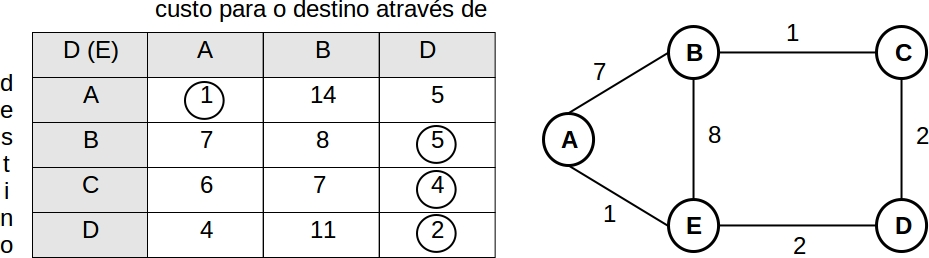
\includegraphics[scale=0.35]{vetor_de_distancia.jpg}
\end{figure}
\begin{itemize}
 \item A partir dos valores selecionados é criada a tabela de roteamento
 \item Periodicamente, cada roteador envia um cópia da sua tabela de roteamento aos roteadores adjacentes % quando ocorre mudanças na rede, stop() quando a ocorre mais troca de mensagem
\end{itemize}
\end{frame}

\begin{frame}{Estado de Enlace}
\begin{itemize}
 \item Cada roteador mantém um representação da topologia da rede na forma de um grafo  % 
\end{itemize}
\begin{figure}[!htb]
\centering
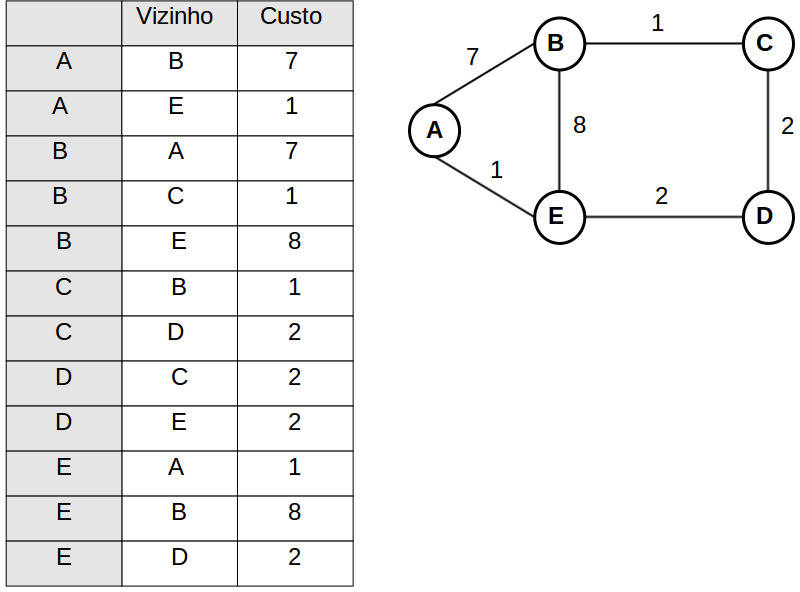
\includegraphics[scale=0.30]{grafo.jpg}
\end{figure}
\end{frame}

\begin{frame}{Estado de Enlace}
Periodicamente, cada roteador:
\begin{itemize}
 \olditem verifica o estado de seus enlaces % através do envio de pequenas mensagens
 \olditem envia as informações do estado dos enlaces aos roteadores adjacentes % quando ocorre mudanças na rede, stop() quando a ocorre mais troca de mensagem
\end{itemize}
\end{frame}

\begin{frame}{Protocolo OSPF}
\begin{itemize}
 \item O \textit{Open Shortest Path First} (OSPF) é um protocolo de roteamento interno % 
 \item Pertence a classe \textbf{estado de enlace} % 
 \item Utiliza o algoritmo de Dijkstra para calcular o caminho mínimo de uma origem para cada destino da rede %
\end{itemize}
\end{frame}

\begin{frame}{Vantagens do OSPF}
\begin{itemize}
 \item Encontra caminhos mínimos de maneira rápida e sem ciclos % pois utiliza o Dijkstra
 \item Utiliza menos largura de banda % pois nao envia a tabela de roteamento inteira, envia somente o estado de seus enlaces 
 \item É possível utilizar diversas métricas no calculo do caminho mínimo % menor custo, maior vazão, maior confiabilidade
 \item Mantém mais de um caminho mínimo para um dado destino % caminhos devem possuir valores de métrica idênticos  % aumenta eficiencia pois possibilita a divisão do trafego 
\end{itemize}
\end{frame}

\begin{frame}{Algoritmo de Dijkstra}
\begin{figure}[!htb]
\centering
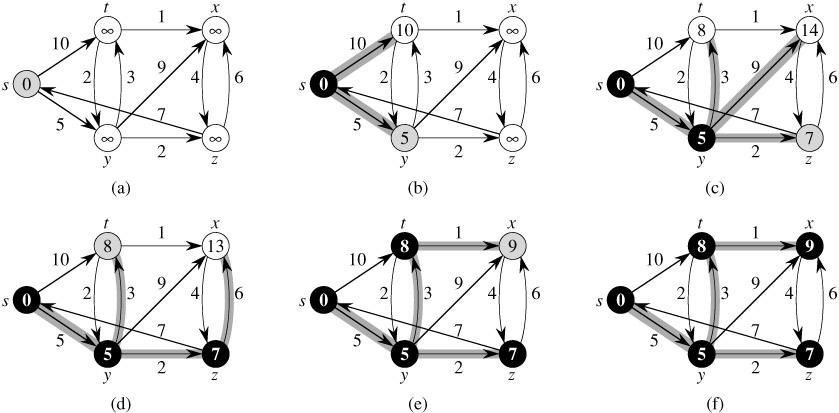
\includegraphics[scale=0.75]{../fig24_6.jpg}
\end{figure}
\end{frame}

\begin{frame}{Protocolo Hello}
\begin{itemize}
 \item Verifica o estado dos enlaces através de pacotes \textit{hello} % identifica falhas
  \begin{enumerate}
   \olditem Cada roteador envia pacotes \textit{broadcast} com uma lista dos vizinhos conhecidos % 
   \olditem Se um vizinho não está na lista então seus pacotes \textit{hello} não foram recebidos % 
   \olditem Então o enlace não é bidirecional e não pode ser usado no roteamento % 
  \end{enumerate}
 \item Elege um roteador \textit{designado} e um roteador \textit{reserva} %  diminui a quantidade de mensagens
  \begin{enumerate}
   \olditem Cada roteador é configurardo com uma prioridade entre 0 e 255 % 
   \olditem Através dos pacotes \textit{hello} os roteadores informam sua prioridade %
   \olditem Normalmente o roteador com maior prioridade é eleito roteador designado % segunda maior prioridade roteador backup
   \olditem Se o roteador designado falha ele é substituído pelo reserva %
  \end{enumerate}
\end{itemize}
\end{frame}

\begin{frame}{Protocolo Exchange}
Quando dois roteadores estabelecem conectividade bidirecional, eles devem sincronizar sua representação local da topologia da rede % 
 \begin{enumerate}
  \olditem Para isso eles trocam pacotes com descrições dos enlaces dos grafo % lista dos enlaces do grafo
  \olditem Em seguida os roteadores solicitam informações de novos enlaces %
  \olditem Por fim os roteadores trocam informações sobre o estado dos enlaces % 
 \end{enumerate}
\end{frame}

\begin{frame}{Protocolo Flooding}
\begin{itemize}
 \item Quando um enlace muda de estado, o roteador responsável por esse enlace deve transmitir uma mensagem com a nova versão do estado do enlace % 
 \item Quando um roteador recebe novas informções sobre o estado de um enlace ele deve atualizar seu grafo e retransmitir as informações  %  
\end{itemize}
\end{frame}

\begin{comment}
\begin{itemize}
 \item  % 
 \item  %  
 \item  % 
 \item  % 
\end{itemize}
\end{comment}

\begin{comment}
\begin{frame}{Belousov–Zhabotinsky}
A reação de Belousov-Zhabotinsky é descrita, de maneira simplificada, como uma
série de reações químicas na forma:

\[ A + B \rightarrow 2A \]
\[ B + C \rightarrow 2B \]
\[ C + A \rightarrow 2C \]

%Nestas equações ocorre a criação de A enquanto não expirar o fornecimento de B,
%e o mesmo ocorre de maneira similar para B e C, de modo que a reação forma um
%ciclo completo.

A fim de promover a difusão da reação, os valores de A, B e C são a média
aritmética das 9 células vizinhas (incluindo a célula central). O novo valor da
célula na posição x, y é calculado ao inserir o valor da média nas equações
acima.
\end{frame}


\begin{frame}[plain]
\begin{table}[h]
\centering
\begin{tabular}{ c c }
t = 0 & t = 50 \\
\includegraphics[scale=0.30]{../imagens/0.png} &
\includegraphics[scale=0.30]{../imagens/50.png} \\
t = 100 & t = 500 \\
\includegraphics[scale=0.30]{../imagens/100.png} &
\includegraphics[scale=0.30]{../imagens/500.png} \\
\end{tabular}
\end{table}
\end{frame}


\begin{frame}[fragile]{Paralelização}
\begin{block}{Inicialização}
O trecho de código responsável por inicializar os valores dos reagentes é paralelizado por
um {\bf \#pragma omp parallel for}.
\end{block}

\begin{lstlisting}
#pragma omp parallel for default(shared) private(x,y,line)
    for(x = 0; x < height; x++) {
        line = x * width;
        for(y = 0; y < width; y++) {
            a[line + y] = drand48();
            b[line + y] = drand48();
            c[line + y] = drand48();
        }
    }
\end{lstlisting}
\end{frame}

\begin{frame}[fragile]{Paralelização}
\begin{block}{Estados do autômato}
O código relacionado ao cálculo de cada estado do autômato celular, também é
paralelizado pelo {\bf \#pragma omp parallel for}.
\end{block}

\begin{lstlisting}
for(t = 0; t < lifetime; t++) {
    #pragma omp parallel for default(none) \
    shared(a,b,c,width,height,lifetime,state,t) \
    private(x,y,c_a,c_b,c_c,i,j,index,line,result)
    for(x = 0; x < height; x++) {
        for(y = 0; y < width; y++) {
            ...
        }
    }
}
\end{lstlisting}
%Nos dois casos o {\it for} escolhido para ser paralelizado foi o mais externo,
%pois deste modo, ocorre o maior ganho de desempenho.
\end{frame}

\begin{frame}{Resultados}
\begin{block}{Hardware Utilizado}
\begin{itemize}
 \item 32 x AMD Opteron(tm) Processor 6136 2.4GHz.
 \item 128 GB de RAM.
\end{itemize}
\end{block}
\begin{table}[h]
\centering
\begin{tabular}{|c|c|c|c|c|}
\hline
Dimensão & Execução & \multicolumn{3}{ c| }{Processadores} \\ \cline{3-5}
& Sequencial & 16 & 8 & 4 \\ \hline
256 x 256 & 22.76s & 2.79s & 3.48s & 6.04s \\
512 x 512 & 1m33.79s & 10.49s & 13.63s & 24.90s \\
1024 x 1024 & 6m26.42s & 35.44s & 56.36s & 1m45.10s \\
2048 x 2048 & 26m14.89s & 2m28.04s & 3m42.04s & 7m00.26s \\
4096 x 4096 & 1h38m07s & 9m47.79s & 15m05.35s & 28m11.05s \\
\hline
\end{tabular}
\caption{Comparação entre o sequencial e OpenMP}
\end{table}
\end{frame}
\end{comment}

\section{O Simulador NS-3} % Descreva o NS-3
\begin{frame}{Simulador NS-3}
\begin{itemize}
 \item O \textit{Network Simulator 3} (NS-3) é um simulador de eventos discretos % 
 \item Voltado principalmente para simulação de redes de computadores %  
 \item É um software livre % 
 \item É construído como um sistema de bibliotecas escritas em C++ % 
\end{itemize}
\end{frame}

\begin{frame}{Instalação}
Os desafios de simular o OSPF já se iniciam na instalação
\begin{itemize}
 \item Três guias de instalação diferentes %  Uma para o somente o NS-3, uma para NS-3 + DCE, uma para NS-3 + DCE + Quagga
  \begin{enumerate}
   \olditem Somente o NS-3 % 
   \olditem O NS-3 e o DCE %
   \olditem O NS-3 e o DCE com suporte para o Quagga % 
  \end{enumerate}
  \begin{itemize}
   \olditem O DCE é um módulo do NS-3 que oferece suporte a aplicações reais % 
   \olditem O Quagga fornece implementações de protocolos de roteamento %
   \olditem O DCE e o Quagga são descritos com mais detalhes a seguir %
  \end{itemize}
 \item São necessários diversos pacotes % 
 \item Cada guia de instalação lista pacotes diferentes % 
 \item Alguns dos pacotes não são listados em nenhuma das guias % 
\end{itemize}
\end{frame}

\begin{comment}
\begin{itemize}
 \item  % 
 \item  %  
 \item  % 
 \item  % 
\end{itemize}
\end{comment}

\begin{comment}
\begin{frame}[fragile]{Paralelização}
\begin{block}{Inicialização}
Para inicializar as matrizes com os reagentes A, B e C foi utilizado o gerador
de números da biblioteca {\it curand}.
\end{block}

\begin{lstlisting}
curandCreateGenerator(&gen, CURAND_RNG_PSEUDO_DEFAULT);
curandSetPseudoRandomGeneratorSeed(gen, time(NULL));
curandGenerateUniform(gen, M.a, M.width * M.height);
curandGenerateUniform(gen, M.b, M.width * M.height);
curandGenerateUniform(gen, M.c, M.width * M.height);
\end{lstlisting}
\end{frame}

\begin{frame}[fragile]{Paralelização}
%A partir da função dim3 foi criada uma abstração de duas dimensões, na qual cada
%bloco tem suas dimensões de acordo com um valor previamente definido, e a
%matriz é divida pela quantidade de blocos necessários para que todas suas
%células sejam atribuídas à uma thread.

\begin{block}{Estados do autômato}
Cada thread calcula o estado de {\bf uma} célula do autômato.
\end{block}

\begin{lstlisting}
dim3 dimBlock(BLOCK_SIZE, BLOCK_SIZE);
dim3 dimGrid(aux, aux);
for(t = 0; t < lifetime; t++) {
    nextState<<<dimGrid, dimBlock>>>(M, state);
    cudaMemcpy(result, M.a, M.size, cudaMemcpyDeviceToHost);
    state = (state + 1) % 2;
}
\end{lstlisting}

\begin{block}{Sincronização}
Após o cálculo de cada estado, é preciso sincronizar todas as threads, isto é
feito pela função cudaMemcpy().
%Além de possibilitar a exibição de cada estado do autômato celular.
\end{block}
\end{frame}

\begin{frame}{Resultados}
\begin{block}{Hardware Utilizado}
\begin{itemize}
 \item 2 x GeForce GTX 480
 \item 8 x Intel(R) Core(TM) i7 3.07GHz.
 \item 12 GB de RAM.
\end{itemize}
\end{block}
\begin{table}[h]
\centering
\begin{tabular}{|c|c|c|c|}
\hline
Dimensão & Execução Sequencial & CUDA & Speedup \\ \hline
256 x 256 & 5.515s & 0.225s & 24 \\
512 x 512 & 21.303s & 0.472s & 45 \\
1024 x 1024 & 1m27.962s & 1.260s & 70 \\
2048 x 2048 & 6m13.430s & 4.305s & 86 \\
3072 x 3072 & 13m13.027s & 9.105s & 87 \\
4096 x 4096 & 23m30.547s & 16.488s & 86 \\
\hline
\end{tabular}
\caption{Speedup do CUDA em relação ao sequencial}
\end{table}
%A partir de 4096 x 4096 o limite de threads é atingido
\end{frame}
\end{comment}

\section{Simulações do OSPF no NS-3} % Detalhe os experimentos que vc fez no NS-3
\begin{frame}{Criar uma simulação}
Criar uma simulação no NS-3 é relativamente simples
\begin{itemize}
 \item Documentação detalhada %  
 \item Diversos exemplos % 
 \item Diversos mecanismos de monitoramento, porém alguns deles exijem determinado nível de conhecimento % 
 \item Oferece alguns desafios como, por exemplo, a documentação sobre falhas de enlace é escassa % 
\end{itemize}
\end{frame}

\begin{frame}{Simulação do OSPF no NS-3}
\begin{itemize}
 \item Em simulações sem falhas o roteamento ocorre de acordo com o esperado %  
 \item Quando ocorre uma falha os pacotes que utilizam o caminho falho não chegam aos seus destinos % 
 \item Não é calculado um novo caminho mínimo % portanto
 \item Os roteadores não são informados sobre a falha do enlace % porque
  \begin{enumerate}
   \olditem Não é implementado o protocolo \textit{Hello} para identificar a falha % 
   \olditem Não é implementado o protocolo \textit{Flooding} para informar todos os roteadores %
  \end{enumerate}
 \item Somente o protocolo \textit{Exchange} está implementado no NS-3 % não é exatamente o exchange mas tem a mesma função
\end{itemize}
\end{frame}

\section{Simulações do OSPF com DCE} % Detalhe os experimentos que vc fez com o DCE
\begin{frame}{O Módulo DCE}
\begin{itemize}
 \item O NS-3 não fornece a implementação completa do OSPF % 
 \item O módulo \textit{Direct Code Execution} (DCE) passa a ser uma alternativa para simular o OSPF %  
 \item O DCE possui a implementação do protocolo OSPF feita pela \textit{Quagga Routing Suite} % 
 \item O DCE também permite utilizar executáveis do sistema operacional Linux % 
\end{itemize}
\end{frame}

\begin{frame}{Quagga Routing Suite}
\begin{itemize}
 \item O Quagga fornece implementações de protocolos de roteamento % 
  \begin{itemize}
   \olditem \textit{Open Shortest Path First} (OSPF) % 
   \olditem \textit{Routing Information Protocol} (RIP) %  
   \olditem \textit{Border Gateway Protocol} (BGP) % 
   \olditem \textit{Intermediate System to Intermediate System} (IS-IS) % 
  \end{itemize}
 \item Esta implementações são para plataformas Unix %  GNU/Linux, Solaris, FreeBSD and NetBSD
\end{itemize}
\end{frame}

\begin{frame}{Simulações}
\begin{itemize}
 \item A maneira de configurar a simulação passa por diversas mudanças quando é utilizado o DCE % 
 \item Grande parte do conhecimento adquirido ao utilizar o NS-3 se torna obsoleto  %  
 \item A documentação do DCE, especialmente a parte relacionada ao OSPF, é insuficiente e incompleta % 
 \item Alguns procedimentos exigem conhecimento de executáveis externos ao NS-3 % por exemplo para configurar as interfaces de rede dos roteadores é preciso conhecer o executável ``ip''
\end{itemize}
\end{frame}

\begin{frame}{Resultados}
\begin{itemize}
 \item Nas simulações sem falhas o roteamento ocorre de acordo com o esperado % 
 \item Nas simulações com falhas é possível perceber que os roteadores percebem a falha do enlace e encontram um novo caminho mínimo %  
 \item Portanto foram usados os protocolo \textit{Hello} e \textit{Flooding} % 
 \item Se existe mais de um caminho de mesmo custo eles são identificados, porém somente um deles é utilizados % 
 \item É possível verificar isso ao utilizar o \textit{tcpdump} para analisar o tráfego de pacotes na rede % 
\end{itemize}
\end{frame}

\begin{frame}[fragile]{Exemplo}
\begin{figure}[!htb]
\centering
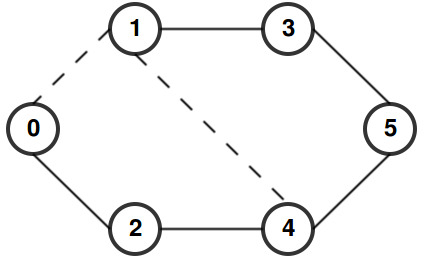
\includegraphics[scale=0.5]{teste1.jpg}
\end{figure}
\end{frame}

\begin{frame}[fragile]{Exemplo}
\begin{figure}[!htb]
\centering
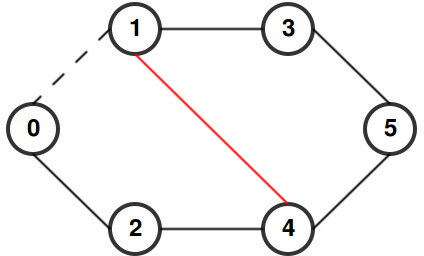
\includegraphics[scale=0.5]{teste2.jpg}
\end{figure}
\begin{itemize}
 \item Falha no enlace 1-4 % 
\end{itemize}
\begin{lstlisting}
RunIp(routers.Get(1), Seconds(74.5), "link set sim2 down");
\end{lstlisting}
\end{frame}

\begin{frame}[fragile]{Exemplo}
\begin{figure}[!htb]
\centering
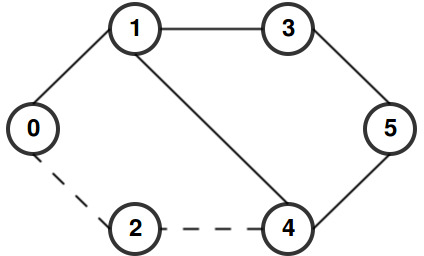
\includegraphics[scale=0.5]{teste3.jpg}
\end{figure}
\end{frame}

\begin{frame}[fragile]{Exemplo}
\begin{itemize}
 \item Último pacote do enlace 1-4 % 
\end{itemize}
\begin{lstlisting}
74.499432 IP 10.0.1.1.57474 > 10.1.4.2.5001: Flags [.], seq 2278929:2280377, ack 1, win 2920, options [nop,nop,TS val 18608 ecr 18607], length 1448
\end{lstlisting}

\begin{itemize}
 \item Enlace 2-4 no momento em que ocorre a falha % 
\end{itemize}

\begin{lstlisting}
65.403112 IP 10.2.4.2 > 224.0.0.5: OSPFv2, Hello, length 48
74.504469 IP 10.2.4.1 > 224.0.0.5: OSPFv2, LS Update, length 76
74.784403 IP 10.0.1.1.57474 > 10.1.4.2.5001: Flags [.], seq 4085885922:4085887370, ack 1742377879, win 2920, options [nop,nop,TS val 18695 ecr 18625], length 1448
\end{lstlisting}
\end{frame}

\begin{frame}[fragile]{Exemplo}
\begin{itemize}
 \item Transferência sem nenhuma falha na rede % 
\end{itemize}
\begin{lstlisting}
Intervalo       Total           Taxa de Transferência
0.0-10.0 seg    5.88 MBytes     4.84 Mbits/seg
\end{lstlisting}

\begin{itemize}
 \item Transferência com a falha na rede % 
\end{itemize}
\begin{lstlisting}
Intervalo       Total           Taxa de Transferência
0.0-10.0 seg    5.62 MBytes     4.70 Mbits/seg
\end{lstlisting}
\end{frame}

\begin{frame}{Dificuldades}
\begin{itemize}
 \item Não foi possível utilizar OSPF em uma rede com enlaces ponto-a-ponto e CSMA % 
  \begin{itemize}
   \olditem Para configurar as interfaces de rede dos roteadores foi utilizado o comando \textit{ip} % documentação focada nos executaveis
   \olditem Este comando tem diversas opções de configuração %  
   \olditem Após diversas tentativas as simulações não estavam ocorrendo de acordo com o esperado % pacotes utilizavam caminhos errados
  \end{itemize}
 \item A última tarefa foi modificar o OSPF, implementado pelo Quagga, para que os roteadores guardassem diversos caminhos, não necessáriamente mínimos, para cada destino %  
   \begin{itemize}
   \olditem O OSPF do Quagga é muito detalhado, uma vez que ele é utilizado em roteadores da Internet % sem abstrações para as simulações
   \olditem Para modifica-lo é preciso compreender detalhes muito específicos  %  
   \olditem Elimina a abstração da simulação % 
  \end{itemize}
\end{itemize}
\end{frame}

\section{Conclusão}
\begin{frame}{Conclusão}
\begin{itemize}
 \item Usar o DCE implica em trabalhar com a própria implementação do protocolo no sistema operacional % 
 \item Elimina a vantagem da simulação, na medida em que múltiplos detalhes devem ser considerados mesmo para testes simples %  
 \item É possível concluir que o trabalho futuro necessário, para permitir a continuidade deste trabalho, é completar a implementação do OSPF nativa do NS-3 % 
\end{itemize}
\end{frame}

\begin{comment}
  \begin{enumerate}
   \olditem Somente o NS-3 % 
   \olditem O NS-3 e o DCE %
   \olditem O NS-3 e o DCE com suporte para o quagga % 
  \end{enumerate}
\begin{itemize}
 \item  % 
 \item  %  
 \item  % 
 \item  % 
\end{itemize}
\end{comment}

\end{document}
